\chapter{\myenchsec{Control Flow} \mymmchsec{ကွန်ထရိုးလ်ဖလိုး}}
\XeTeXlinebreaklocale "my_MM"  %Myanmar line and character breaks
\XeTeXinterwordspaceshaping=2
\begin{sloppypar}
ကားရဲလ်ကို ရှေ့ကို ၂၅ လှမ်း ရွှေ့ခိုင်းချင်တယ်။ \mycode{move(); move(); move(); ...move();} ၂၅ ခါ ရေးလို့‌တော့ရတာပေါ့။ ဒါပေမယ့် စာရိုက်ရတာ အချိန်လည်းကုန် လက်လဲညောင်း ဖြစ်မယ်။ {\mycode{move();}} ကို ၂၅ ကြိမ် ကျော့ပေးပါလို့ ခိုင်းလို့ရရင် ပိုမကောင်းဘူးလား။ 

ကားရဲလ်ရဲ့ ရှေ့တည့်တည့် ခပ်လှမ်းလှမ်းမှာ နံရံတစ်ခုရှိနေမယ်။ ဘယ်လောက်ဝေးလဲ မသိဘူးဆိုပါစို့။ ကားရဲလ်ကို နံရံဆီရောက်အောင် သွားခိုင်းချင်တယ်။ နံရံက ဘယ်လောက်ဝေးလဲ မသိတော့ {\mycode{move}} ကို ဘယ်နှစ်ကြိမ် ကျော့ခိုင်းရမလဲ မသိနိုင်ဘူး။ ရှေ့မှာရှင်းနေသေးသ၍ \mycode{move} ပါလို့သာ ခိုင်းလို့ရမယ်ဆိုရင် တော်တော်လေး အဆင်ပြေပြီ။  

အခြေအနေတစ်ခု မှန်တော့မှပဲ \mmcommand တွေကို  လုပ်ဆောင်စေချင်တာမျိုးလဲ ရှိတယ်။ အဲဒီ အခြေနေနဲ့ မကိုက်ညီဘူး (တနည်းအားဖြင့် အခြေအနေက မှားနေခဲ့ရင်) \mmcommand တွေကို မလုပ်ဆောင်ပဲ ကျော်သွားစေချင်တယ်။ ရှေ့မှာပြောခဲ့တဲ့ နံရံအောက််ခြေမှာ \mmbeeper တစ်ခု ရှိနေနိုင်တယ်၊ ရှိချင်မှလည်း ရှိမယ်ဆိုပါစို့။ \mmbeeper ရှိနေခဲ့ရင် နံရံ အခြားတဘက်မှာ \mmbeeper ကို ထားခိုင်းချင်တယ်။  ဒါဆိုရင် \mmbeeper ရှိနေမှပဲ အခြားတဘက်ကို ရွှေ့ခိုင်းဖို့ လိုအပ်တဲ့ \mmcommand တွေကို လုပ်ဆောင်စေချင်တယ်။ \mmbeeper မရှိဘူးဆိုရင် အဲဒီ \mmcommand တွေကို မလုပ်ဆောင်စေချင်ဘူး။  

နောက်ထပ်တစ်မျိုးက အခြေအနေတစ်ခု မှန်ခဲ့ရင် လုပ်ဆောင်စေချင်တဲ့ \mmcommand တွေနဲ့ မှားခဲ့ရင်‌ လုပ်ဆောင်စေချင်တဲ့ \mmcommand ‌တွေကို မတူပဲဖြစ်နေတာမျိုးပါ။ တနည်းအားဖြင့် အခြေအနေပေါ် မူတည်ပြီး ခိုင်းရမယ့် အလုပ်ကမတူဘူး။ \mmbeeper ရှိခဲ့ရင် နံရံရဲ့ အခြားဘက်ကိုရွှေ့ခိုင်းချင်တယ်၊ မရှိခဲ့ရင်တော့ လာလမ်းအတိုင်း ပြန်လာစေချင်တယ် ဆိုပါစို့။ ဒါဆိုရင် \mmbeeper ရှိခြင်း၊ မရှိခြင်းပေါ် မူတည်ပြီး လုပ်ဆောင်ရမယ့် \mmcommand တွေက  မတူဘူး။ 

ဒီအခန်းမှာတော့ အထက်ပါ လိုအပ်ချက်မျိုးတွေအတွက် အသုံးပြုတဲ့ \enControlFlowStatements တွေကို လေ့လာကြမယ်။ ပြန်ကျော့ဖို့အတွက် သုံးတဲ့ \mycode{for} \myen{loop} နဲ့ \mycode{while} \myen{loop} ကို အရင်ကြည့်ကြရအောင်။

\section{{\mycodesecttl{for}} \myensecttl{loop}}
\mycode{for} \myen{loop} ကို \mmcommand တစ်ခု သို့ တစ်စုကို ပြန်ကျော့ဖို့ အသုံးပြုနိုင်တယ်။ \mmsyntax က အခုလိုပုံစံမျိုး နဲ့ရေးရတယ်  
\begin{lstcodeminimal}
for (int i = 0; i < N; i++) {
    //one or more commands here
}
\end{lstcodeminimal}
\mycode{move} ကို နှစ်ဆယ့်ငါးကြိမ် ကျော့ချင်ရင် 
\begin{lstcodeminimal}[]
for (int i = 0; i < 25; i++) {
    move();
}
\end{lstcodeminimal}
ပြန်ကျော့ချင်တဲ့ \mmcommand တွေကို \mmcurlybrpair အတွင်း လိုင်းတွေမှာရေးပြီး \mycode{N} နေရာမှာ အကြိမ်အရေအတွက်ကို အစားထိုးပေးရမယ်။ \mycode{int i} မှာ ခြားထားရပါမယ်။ \mycode{inti} ဆိုရင် \mmsyntaxerr ဖြစ်မယ်။ \mycode{i++} က တဆက်ထဲ ဖြစ်ရမယ်။ \mycode {i ++} သို့ \mycode {i + +} သို့ \mycode {i+ +} ရေးလို့ မရဘူး။ ကျန်တဲ့ စပေ့စ်တွေက ခြားသည်ဖြစ်စေ မခြားသည်ဖြစ်စေ ပြဿနာ \mmsyntax\ အရတော့ မှန်တယ်။ ဒီလိုရေးလို့ ရပေမယ့် ဖတ်ရတာ ခက်တယ်။ 
\begin{lstcodeminimal}[]
for (int i=0;i<25;i++){
move();
}
\end{lstcodeminimal}
\noindent ပူးကပ်နေပြီး အမြင်အရလည်း မရှင်းလင်းဘူး။

\subsection{\mycodesubsecttl{for} \myensubsecttl{loop} အသုံးပြုသည့် ဥပမာများ}
\begin{figure}[htb]
    \caption{ကားရဲလ်နှင့်  ကားရဲလ်၏ကမ္ဘာ}\label{fig:MakeRowOfFiveBeepersInit}
    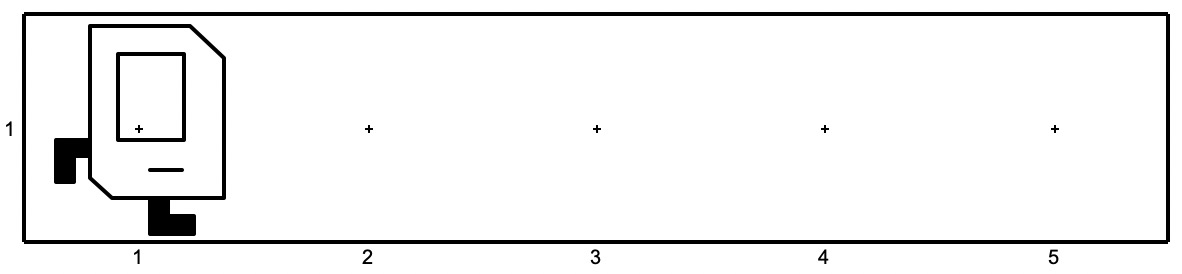
\includegraphics[scale=0.2, left]{ch02/MakeRowOfFiveBeepers/init.jpg}
\end{figure}
ကားရဲလ်က \Fig \vref*{fig:MakeRowOfFiveBeepersInit} ကမ္ဘာထဲမှာရှိနေမယ်။ လမ်းတလျှောက်လုံး \mmcorner တစ်ခု စီတိုင်းမှာ \mmbeeper တစ်ခု ချထားခိုင်းချင်တယ်။ \mmavenue အရေအတွက်က ဒီပုစ္ဆာအတွက် အပြောင်းအလဲမရှိဘူး။ ပုံသေ ၅ ခုပဲဖြစ်မယ်လို့ ယူဆပါ။ \mmbeeper ချလိုက် ရှေ့\mmcorner ကို ရွှေ့လိုက်၊ \mmbeeper ချလိုက် ရှေ့\mmcorner ကို ရွှေ့လိုက် လုပ်ခိုင်းရမှာပေါ့။  ပြန်ကျော့ပေးရမယ့် \mmcommand နှစ်ခုက \mycode{putBeeper} နဲ့ \mycode{move}။ ဘယ်နှစ်ကြိမ် ကျော့ခိုင်းရမှာလဲ။ သေချာဖို့လိုတယ်။ သေချာတာက ကားရဲလ်ရှေ့မှာ \mmcorner လေးခုပဲရှိတဲ့အတွက် ရှေ့ကို လေးနေရာပဲ ရွှေ့လို့ရမယ်။ \mycode{N} နေရာမှာ \mycode{4} ထည့်ပြီး အခုလို ရေးရမယ်။ \Lst \vref*{lst:MakeRowOfFiveBeepersOffByOne} တွင်ကြည့်ပါ။

 % Ex -> start with putBeeper
\begin{lstcodesimple}[float, caption=ပထမစမ်းကြည့်ပုံ, label={lst:MakeRowOfFiveBeepersOffByOne}]
public class MakeRowOfFiveBeepers extends stanford.karel.Karel{
    public void run(){
            for(int i = 0; i < 4; i++) {
                    putBeeper();
                    move();
            }
    }
}
\end{lstcodesimple}

ဒီတိုင်း \mmrun ကြည့်တဲ့ရအောင်။ ရလဒ်ကို \Fig \vref{fig:MakeRowOfFiveBeepersOffByOne} တွင်ကြည့်ပါ။  နောက်ဆုံး \mmcorner မှာ \mmbeeper ချဖို့ကျန်နေတာ တွေ့ရမယ်။ ဘာကြောင့်ကျန်နေရတာလဲ။ သေချာ နားလည်အောင် \mmiteration တစ်ခါပြီးတိုင်း ရှိနေမယ့် အခြေအနေကို \vref*{fig:MakeRowOfFiveBeepersIters} မှာကြည့်ပါ။ နောက်ဆုံး \mmcorner မှာ \mmbeeper ချပေးဖို့အတွက် \mycode{for} \myen{loop} \mmClosingCurlyBrace\ နောက်တစ်လိုင်းမှာ \mycode{putBeeper();} \mmcommand ရေးပေးရမယ်။ \enForLoopBody အပြင်မှာရှိတဲ့အတွက် ပြန်ကျော့မယ့် \mmcommand\ ထဲမှာ မပါဘူး။ နောက်ဆုံးမှာ တစ်ကြိမ်ပဲ လုပ်ဆောင်တယ်။ \Lst \vref*{lst:MakeRowOfFiveBeepersFixedOffByOne} တွင်ကြည့်ပါ။

\begin{figure}[htb]
    \caption{ကားရဲလ်နှင့်  ကားရဲလ်၏ကမ္ဘာ}\label{fig:MakeRowOfFiveBeepersOffByOne}
    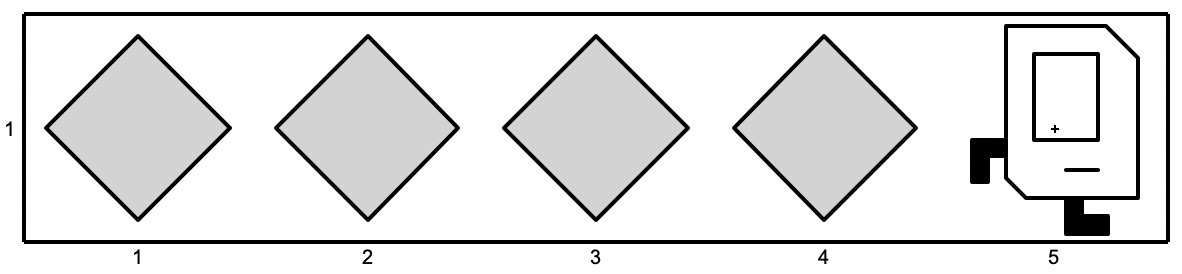
\includegraphics[scale=0.2, left]{ch02/MakeRowOfFiveBeepers/off_by_one_1.jpg}
\end{figure}

\begin{figure}[tbh!]
    \begin{subfigure}[t]{0.8\textwidth}
        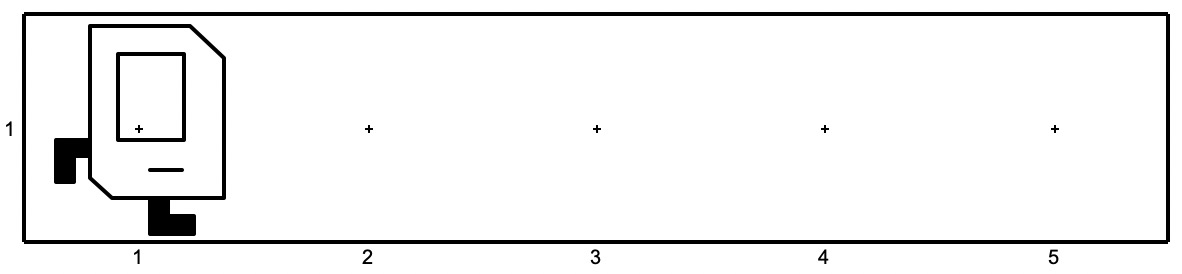
\includegraphics[scale=0.2, left]{ch02/MakeRowOfFiveBeepers/init.jpg}
        \caption{မူလ အနေအထား}    
    \end{subfigure}
    \begin{subfigure}[t]{0.8\textwidth}
        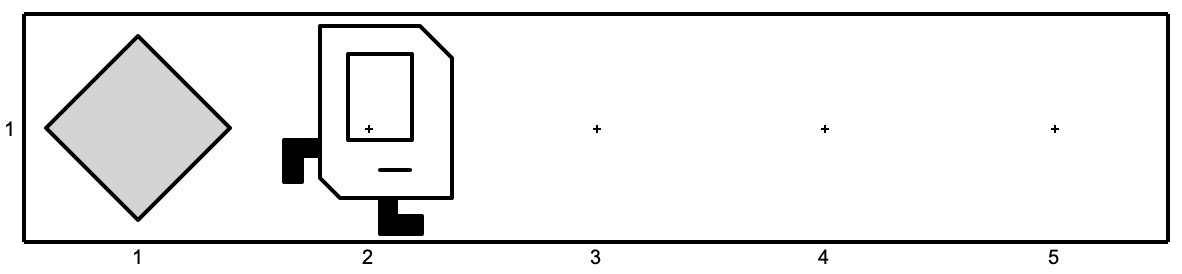
\includegraphics[scale=0.2, left]{ch02/MakeRowOfFiveBeepers/1st_iter.jpg}
        \caption{ပထမ တစ်ကျော့ပြီး}    
    \end{subfigure}
    \begin{subfigure}[t]{0.8\textwidth}
        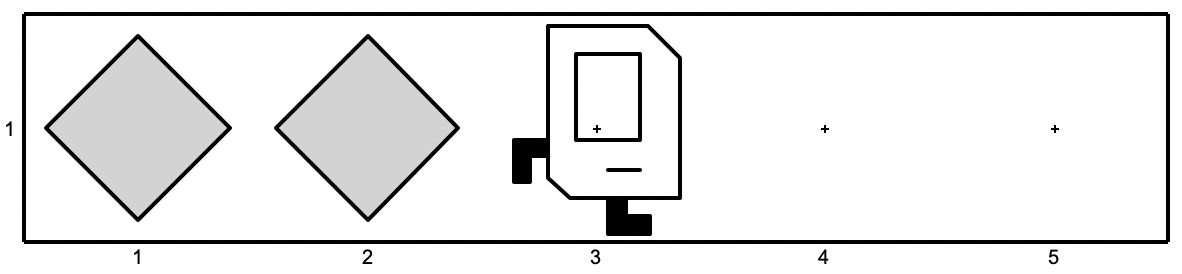
\includegraphics[scale=0.2, left]{ch02/MakeRowOfFiveBeepers/2nd_iter.jpg}
        \caption{ဒုတိယ တစ်ကျော့ပြီး}    
    \end{subfigure}
    \begin{subfigure}[t]{0.8\textwidth}
        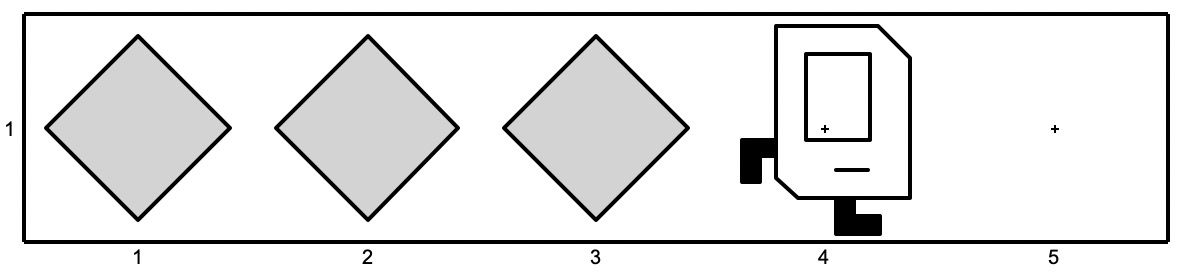
\includegraphics[scale=0.2, left]{ch02/MakeRowOfFiveBeepers/3rd_iter.jpg}
        \caption{တတိယ တစ်ကျော့ပြီး}    
    \end{subfigure}
    \begin{subfigure}[t]{0.8\textwidth}
        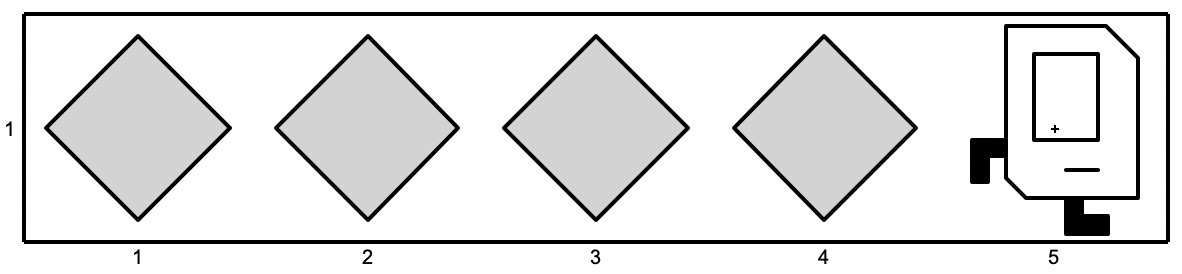
\includegraphics[scale=0.2, left]{ch02/MakeRowOfFiveBeepers/4th_iter.jpg}
        \caption{စတုတ္ထမြောက် ကျော့ပြီး}    
    \end{subfigure}
    \caption{\mmiteration တစ်ခုပြီး}
    \label{fig:MakeRowOfFiveBeepersIters}
\end{figure}

\begin{lstcodesimple}[float, caption={ပထမစမ်းကြည့်ပုံ}, 
                        label={lst:MakeRowOfFiveBeepersFixedOffByOne}]
public class MakeRowOfFiveBeepers extends stanford.karel.Karel{
    public void run(){
            for(int i = 0; i < 4; i++) {
                    putBeeper();
                    move();
            }

            putBeeper();
    }
}
\end{lstcodesimple}

\Fig \vref{subfig:MakeBeeperSquareInit} မှ စတုရန်းပုံ ကမ္ဘာထဲမှာ \mmcorner တွေမှာ \mmbeeper တစ်ခုစီ ချဖို့ \enForLoop ကိုသုံးနိုင်တယ်။  \Lst \vref*{lst:MakeBeeperSquare} တွင်ကြည့်ပါ။ \mmiteration တစ်ခါတိုင်းမှာ 
\begin{lstcodeminimal}[]
putBeeper();
move();
turnLeft();    
\end{lstcodeminimal}

\noindent ကို လုပ်ဆောင်မှာဖြစ်တယ်။ တစ်ကြိမ်ကျော့အပြီးမှာ ရှိနေမယ့် အခြေအနေကို \Fig \vref*{fig:MakeBeeperSquareIters} တွင်ကြည့်ပါ။
\begin{lstcodesimple}[float, caption={စတုရန်းပုံ ဘိပါ}, label={lst:MakeBeeperSquare}]
public class MakeBeeperSquare extends stanford.karel.Karel{
        public void run(){
                for(int i = 0; i < 4; i++) {
                        putBeeper();
                        move();
                        turnLeft();
                }
        }
}
\end{lstcodesimple}

\begin{figure}[tbh!]
    \caption{\myenlstcpt{Beeper Seqare}}
    \begin{subfigure}[t]{0.46\textwidth}
        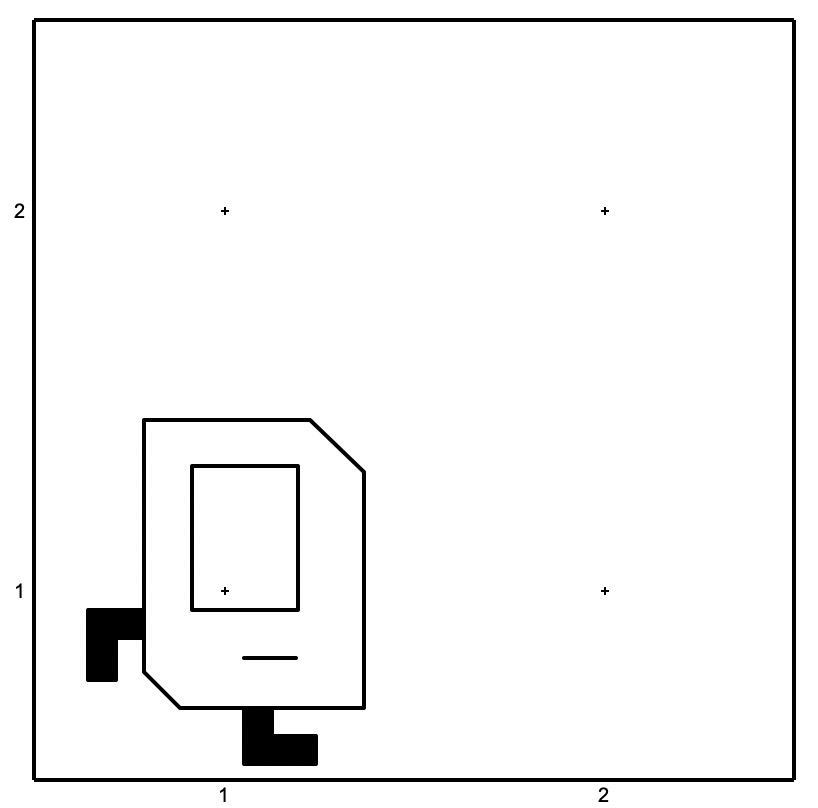
\includegraphics[scale=0.17, left]{ch02/MakeBeeperSquare/init.jpg}
        \caption{ကနဦး အနေအထား}
        \label{subfig:MakeBeeperSquareInit}
    \end{subfigure}
    \hspace{0.1in}
    \begin{subfigure}[t]{0.46\textwidth}
        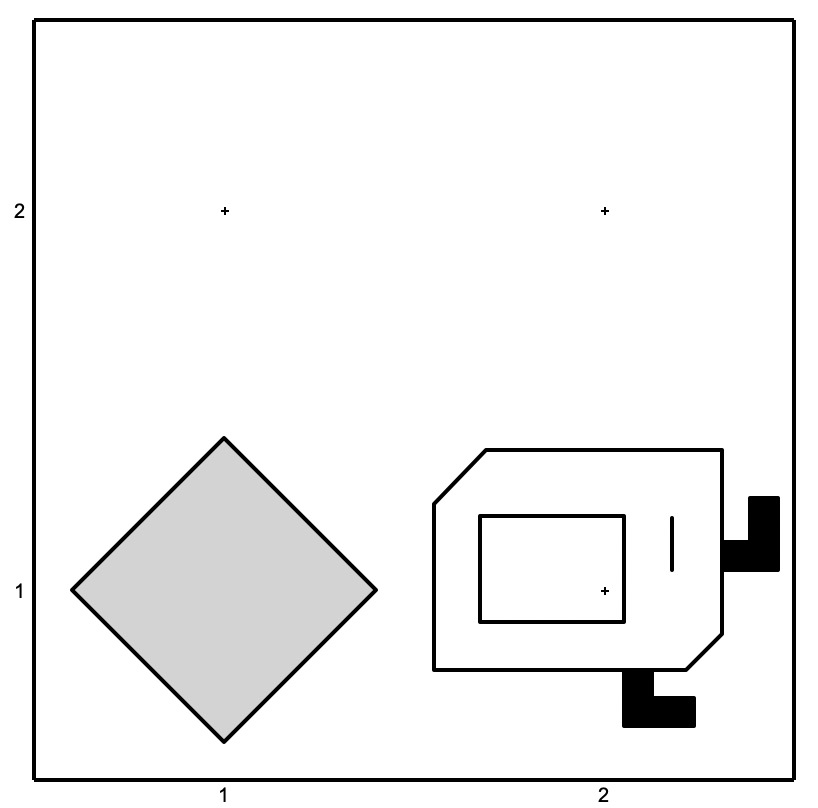
\includegraphics[scale=0.17, left]{ch02/MakeBeeperSquare/1st_iter.jpg}
        \caption{\myttlcode{move} \mmcommand လုပ်ဆောင်ပြီး}
    \end{subfigure}

    \begin{subfigure}[t]{0.46\textwidth}
        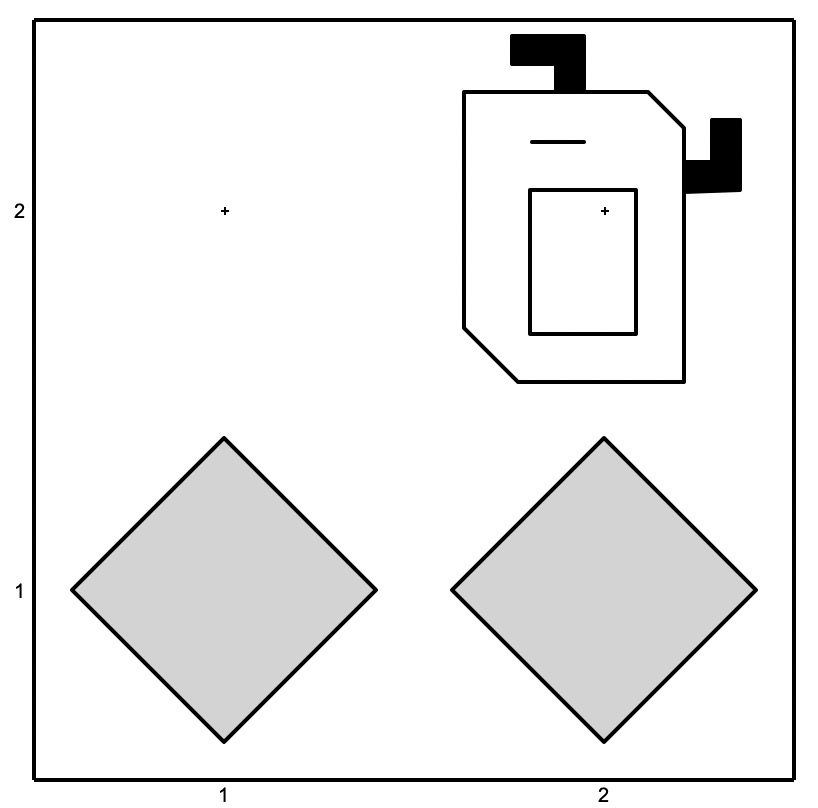
\includegraphics[scale=0.17, left]{ch02/MakeBeeperSquare/2nd_iter.jpg}
        \caption{ကနဦး အနေအထား}
    \end{subfigure}
    \hspace{0.1in}
    \begin{subfigure}[t]{0.46\textwidth}
        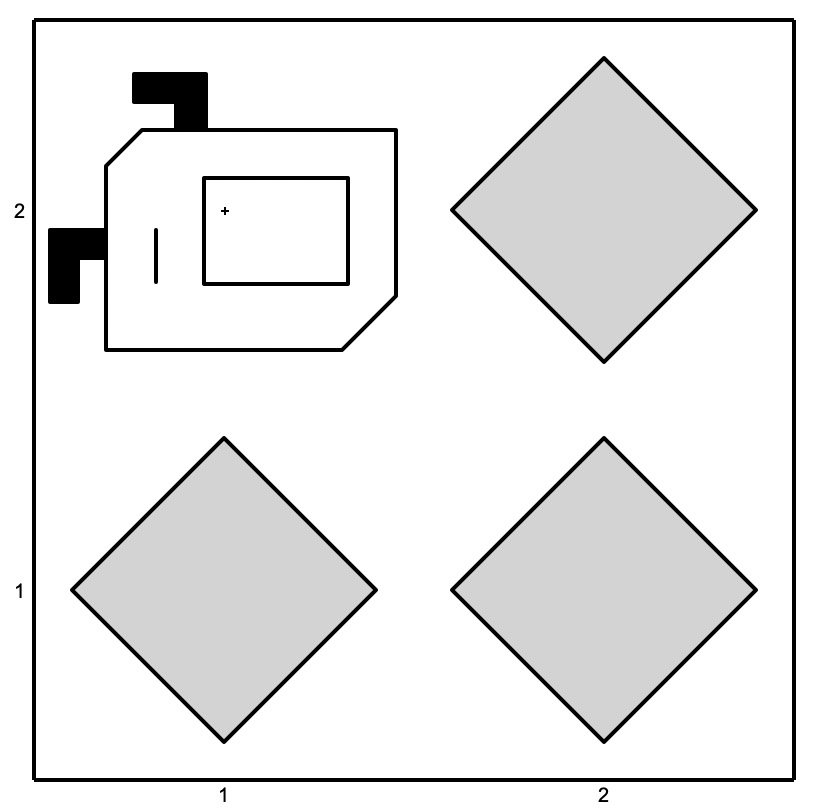
\includegraphics[scale=0.17, left]{ch02/MakeBeeperSquare/3rd_iter.jpg}
        \caption{\myttlcode{move} \mmcommand လုပ်ဆောင်ပြီး}
    \end{subfigure}

    \begin{subfigure}[t]{0.46\textwidth}
        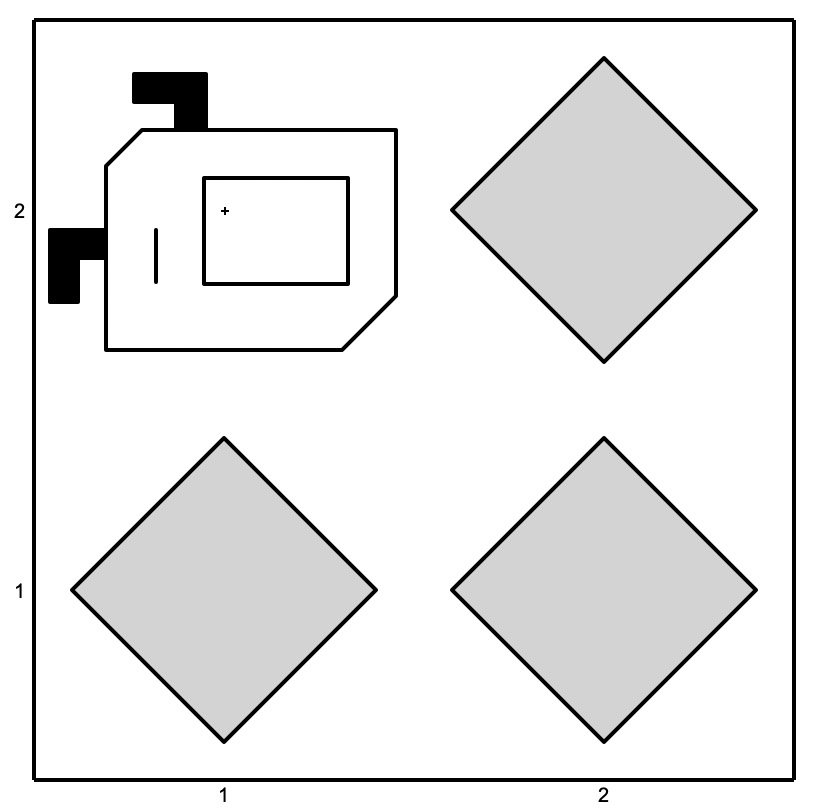
\includegraphics[scale=0.17, left]{ch02/MakeBeeperSquare/3rd_iter.jpg}
        \caption{\myttlcode{move} \mmcommand လုပ်ဆောင်ပြီး}
    \end{subfigure}
    \hspace{0.1in}
    \label{fig:MakeBeeperSquareIters}
\end{figure}



\section{\mycodesecttl{while} \myensecttl{loop}}
အကြိမ်အရေအတွက် မသိပဲ အခြေအနေတစ်ခု မှန်နေသ၍ ပြန်ကျော့ဖို့ \enWhileLoop ကို သုံးတယ်။ \mmsyntax က အောက်ပါအတိုင်းရေးတယ်။  
\begin{lstcodeminimal}
while (CONDITION) {
    //commands to be executed while condition is true
}
\end{lstcodeminimal}
\myen{condition} နေရာမှာ \vref*{tbl:KarelConditions} ပါ \mmCondition တစ်ခုကို အစားထိုးပေရမှာပါ။ ရှေ့မှာ ရှင်းနေသ၍ ရွှေ့ခိုင်းချင်တယ် ဆိုရင်
\begin{lstcodeminimal}
while (frontIsClear()) {
    move();
}
\end{lstcodeminimal}

\subsection{\mycodesecttl{while} \myensecttl{loop} အသုံးပြုသည့် ဥပမာများ}
ကားရဲလ် အရှေ့ဘက်မှာ အုန်းပင်တစ်ပင်ရှိတယ်။ ဘယ်လောက်အကွာအဝေးမှာ ရှိနေမလဲ ပုံသေပြောလို့မရဘူး။ နမူနာ နှစ်ခုကို ပုံမှာပြထားတယ်။ က မှာရှိနေသည်ဖြစ်စေ၊ ခ မှာရှိနေသည်ဖြစ်စေ၊ နံရံဆီကို သွားခိုင်းရမယ်။ ဒါ့အပြင် နောက်ထပ် အလားတူတဲ့  အခြားကမ္ဘာတွေထဲမှာလည်း နံရံက ဘယ်လောက်အကွာအဝေးမှာ ရှိနေသည်ဖြစ်စေ ကားရဲလ်ကို ရောက်အောင် သွားခိုင်းချင်တယ်။ 

\begin{figure}[tbh!]
    \caption{\myenlstcpt{CococonutTree}}
    \begin{subfigure}[t]{0.46\textwidth}
        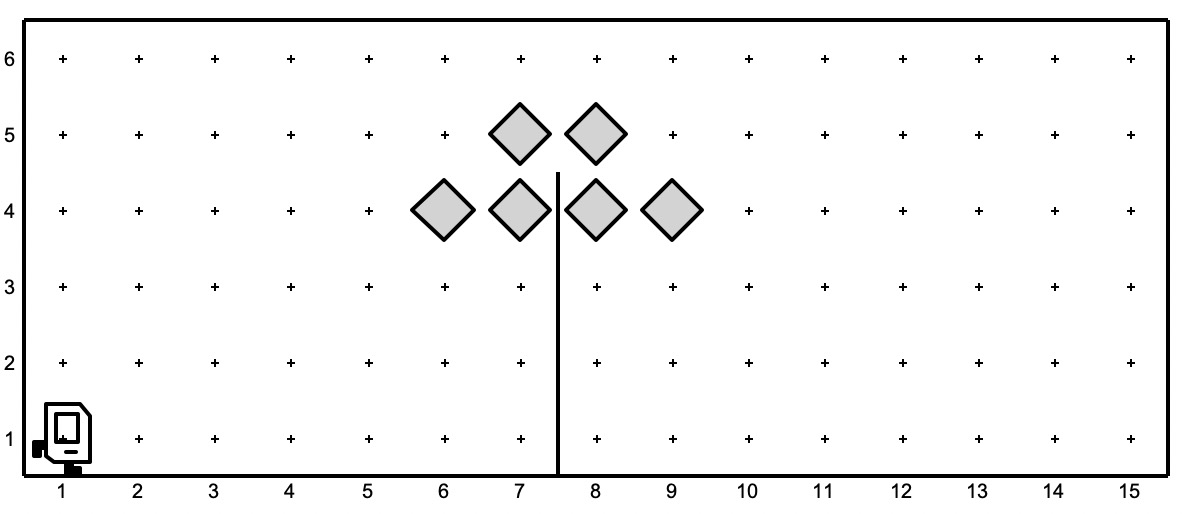
\includegraphics[height=2.2in, left]{ch02/CoconutTree/a.jpg}
        \caption{}
        \label{subfig:CoCoconutTreeA}
    \end{subfigure}

    \begin{subfigure}[t]{0.46\textwidth}
        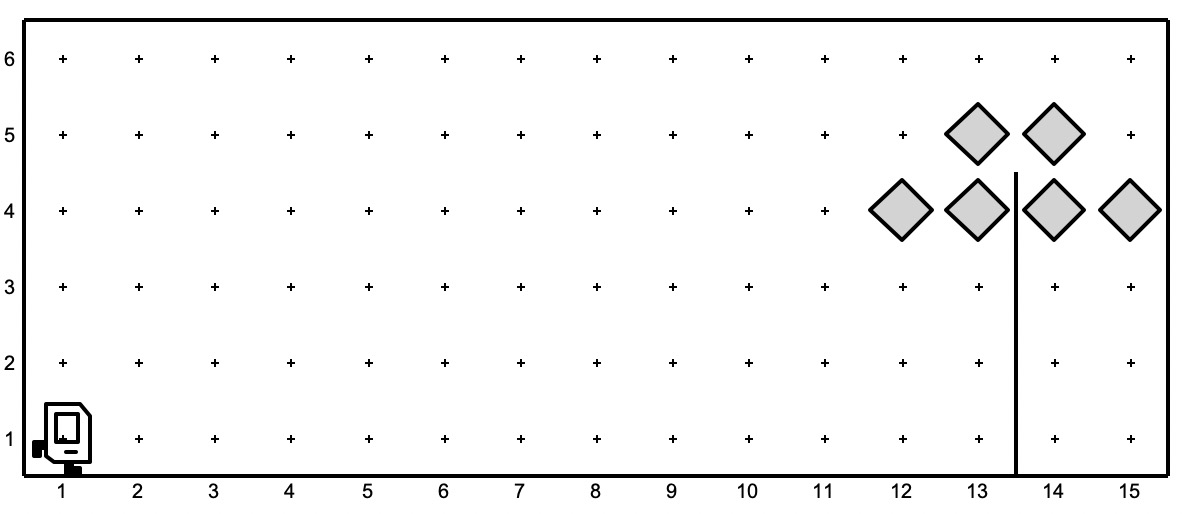
\includegraphics[height=2.2in, left]{ch02/CoconutTree/b.jpg}
        \caption{}
    \end{subfigure}
\end{figure}

\begin{lstcodesimple}[float, caption={\mycodelstcpt{CococonutTree.java} \myenlstcpt{A}}, label={lst:CococonutTree}]
public class CococonutTree extends stanford.karel.Karel{
    public void run(){
            while(frontIsClear()){
                    move();
            }
    }
}
\end{lstcodesimple}

နောက်ထပ် ဥပမာတစ်ခု ကြည့်ရအောင်။ ကားရဲလ်ကို လမ်းတလျှောက် \mmbeeper  တွေချထားခိုင်းချင်တယ်။ လမ်းအရှည်က ဘယ်လောက်ဖြစ်ဖြစ် အပြည့်ချထားပေးရမယ်။ လမ်းအရှည်က ပုံသေမဟုတ်တဲ့အတွက် ရှေ့မှာရှင်းနေသ၍ \mmbeeper ချလိုက် ရှေ့တိုးလိုက် ထပ်ခါထပ်ခါ လုပ်ခိုင်းရမှာပေါ့။ 

\begin{lstcodesimple}[float, caption={\mycodelstcpt{MakeBeeperRow.java} \myenlstcpt{A}}, label={lst:MakeBeeperRow}]
public class MakeBeeperRow extends stanford.karel.Karel{
    public void run(){
            while(frontIsClear()){
                    putBeeper();
                    move();
            }
            putBeeper();
    }
}
\end{lstcodesimple}

\enForLoop မှာလိုပဲ \myen{loop} \mmBody ကို နောက်ဆုံးအကြိမ် လုပ်ဆောင်အပြီးမှာ \mmbeeper ချဖို့ကျန်နေမယ်။ ဒါကြောင့် \enWhileLoopBody နောက်တစ်လိုင်းမှာ \mycode{putBeeper();} ပါရမှာဖြစ်တယ်။

\begin{figure}[tbh!]
    \caption{\myenlstcpt{MakeBeeperRow}}
    \begin{subfigure}[t]{0.46\textwidth}
        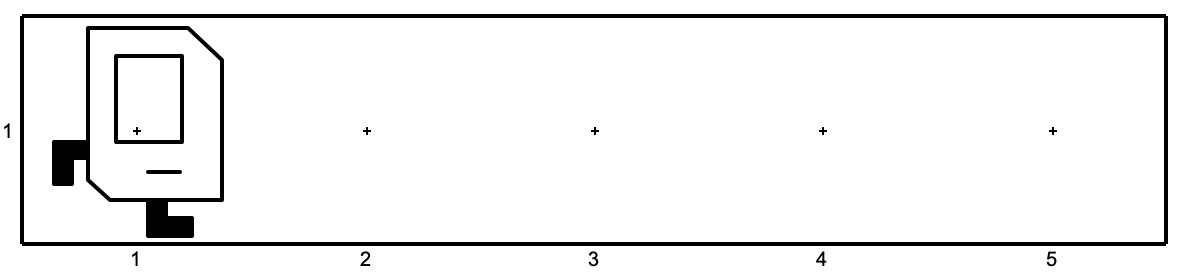
\includegraphics[width=2.75in, left]{ch02/MakeBeeperRow/init.jpg}
        \caption{}
        \label{subfig:MakeBeeperRowA}
    \end{subfigure}

    \begin{subfigure}[t]{0.46\textwidth}
        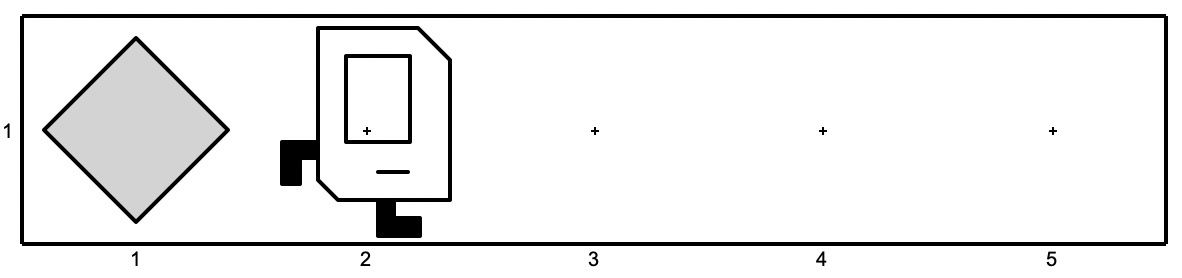
\includegraphics[width=2.75in, left]{ch02/MakeBeeperRow/1st_iter.jpg}
        \caption{}
    \end{subfigure}

    \begin{subfigure}[t]{0.46\textwidth}
        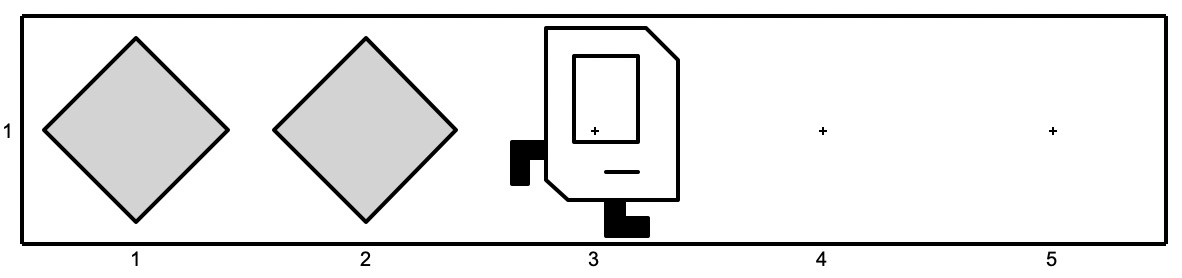
\includegraphics[width=2.75in, left]{ch02/MakeBeeperRow/2nd_iter.jpg}
        \caption{}
    \end{subfigure}

    \begin{subfigure}[t]{0.46\textwidth}
        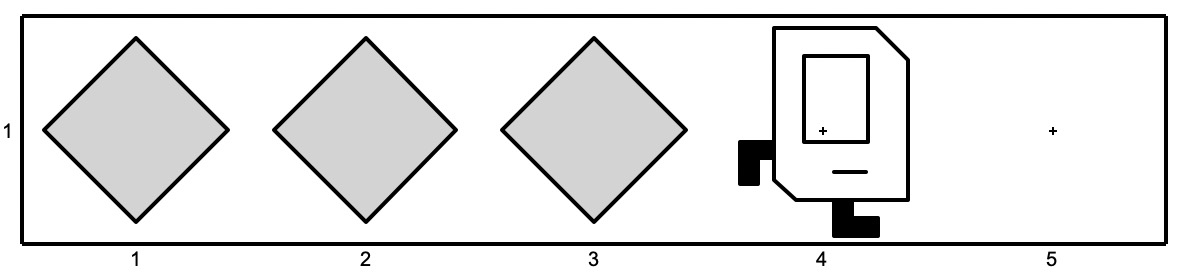
\includegraphics[width=2.75in, left]{ch02/MakeBeeperRow/3rd_iter.jpg}
        \caption{}
    \end{subfigure}

    \begin{subfigure}[t]{0.46\textwidth}
        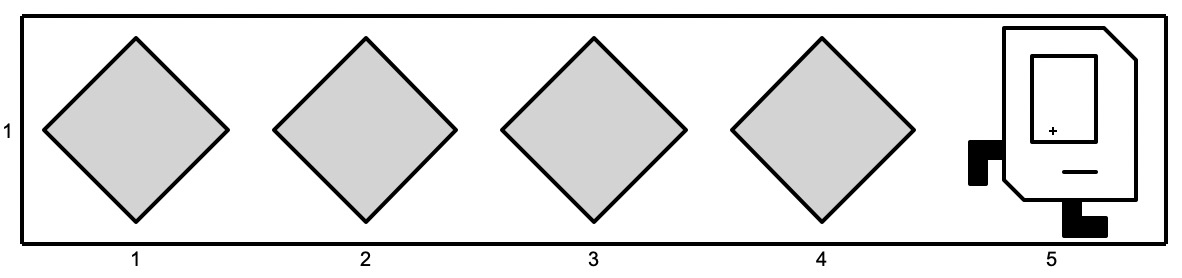
\includegraphics[width=2.75in, left]{ch02/MakeBeeperRow/4th_iter.jpg}
        \caption{}
    \end{subfigure}
    \label{fig:MakeBeeperRowIters}
\end{figure}

\enWhileLoop အလုပ်လုပ်ပုံက အခုလိုပါ။  \mmCondition ကို အရင်ဆုံး စစ်ပါတယ်။ မှန်လျှင် \mmBody ထဲက \mmcommand တွေကို လုပ်ဆောင်တယ်။ တစ်ကြိမ်ကျော့ပြီးတိုင်း \mmCondition ကိုပြန်စစ်ပါတယ်။ မှန်နေသေးလျှင် \mmBody ထဲက \mmcommand တွေကို ထပ်ပြီးကျော့ပေးပါတယ်။ ဒီလိုမျိုး \mmCondition စစ်လိုက်၊ မှန်နေရင် ပြန်ကျော့လိုက်ကို ထပ်ခါထပ်ခါ လုပ်နေပြီး \mmCondition စစ်လိုက်လို့ မှားနေတဲ့ အခါကျတော့မှ ပြန်ကျော့တာကို ရပ်လိုက်တာဖြစ်တယ်။ ပြန်ကျော့တာရပ်လိုက်တာကို \enLoopExits တယ်လို့ ပြောလေ့ရှိတယ်။

\mmLoopExits သွားပြီးနောက် \mmLoopBody ‌အောက်ကမှာရှိတဲ့လိုင်းတွေကို ဆက်ပြီးလုပ်ဆောင်မှာ ဖြစ်တယ်။ ရှေ့ကဥပမာမှာ လေးကြိမ်မြောက်ထိ \mycode{frontIsClear} \mmCondition က မှန်နေတယ်။ ဒါကြောင့် လေးခါကျော့ ခံရမယ်။ ငါးကြိမ်မြောက် \mmCondition စစ်တဲ့အခါမှာတော့ \mycode{frontIsClear} ကမှားနေပြီ။ ရှေ့မှာ နံရံပိတ်နေတယ်။ ထပ်မကျော့တော့ပဲ \mmLoopExits ပြီး နောက်တလိုင်းက \mycode{putBeeper();} ကို ဆက်လက်လုပ်ဆောင်တယ်။

\enWhileLoop \mmCondition က ဘယ်တော့မှ မမှားတော့ပဲ အမြဲမှန်နေတာမျိုးရှိနိုင်တယ်။ ဒီအခါမှာတော့ \enLoop ထဲကနေ ဘယ်တော့မှ ထွက်မသွားတော့ပဲ \mmBody ထဲက \mmcommand တွေကို ထာဝရ လုပ်ဆောင်နေတော့မှာ ဖြစ်တယ်။ ဒီလို အစဉ်အမြဲ ပြန်ကျော့နေမယ့် \mmLoop ကို \mmInfiniteLoop လို့ခေါ်ပါတယ်။ \enInfiniteLoop ထဲကနေ မထွက်တော့တဲ့ အတွက် \mmLoopBody အောက် လိုင်းတွေမှာရှိတဲ့ \mmcommand တွေကိုလည်း လုပ်ဆောင်မှာ မဟုတ်ပါဘူး။ 

\noindent \Lst \vref*{lst:GoAroundForever} မှာ \mycode{pickBeeper();} ကို ဘယ်တော့မှ လုပ်ဆောင်ဖြစ်မှာ မဟုတ်ပါဘူး။

\begin{lstcodesimple}[float, caption={\mycodelstcpt{GoAroundForever.java} \myenlstcpt{A}}, label={lst:GoAroundForever}]
public class GoAroundForever extends stanford.karel.Karel{
    public void run(){
            //Karel will never get out of this loop
            while(frontIsClear()) {
                    move();
                    turnLeft();
            }
            //This command will never be executed
            pickBeeper();
    }
}
\end{lstcodesimple}

\enWhileLoop \enCondition က ပထမဆုံး စစစ်လိုက်တဲ့ အခါမှာပဲ မှားနေရင် \mmcommand တွေကို တစ်ခါမှ မကျော့ပေးတော့ပဲ \mmLoopExits မှာဖြစ်တယ်။ ဒါကိုတော့ \enLoopNeverEntered လို့ပြောလေ့ရှိတယ်။

\begin{lstcodesimple}[float, caption={\mycodelstcpt{LoopNeverEntered.java} \myenlstcpt{A}}, label={lst:LoopNeverEntered}]
public class LoopNeverEntered extends stanford.karel.Karel{
    public void run(){
            // This loop is never entered for default world
            // and its body will be totally skipped
            while(frontIsClear()) {
                    move();
                    turnLeft();
                    putBeeper();
            }
            // Commands below will be executed as usual
            turnLeft();
            move();
            putBeeper();
    }
}
\end{lstcodesimple}

\begin{figure}[tbh!]
    \caption{\myenlstcpt{LoopNeverEntered}}
    \begin{subfigure}[t]{0.46\textwidth}
        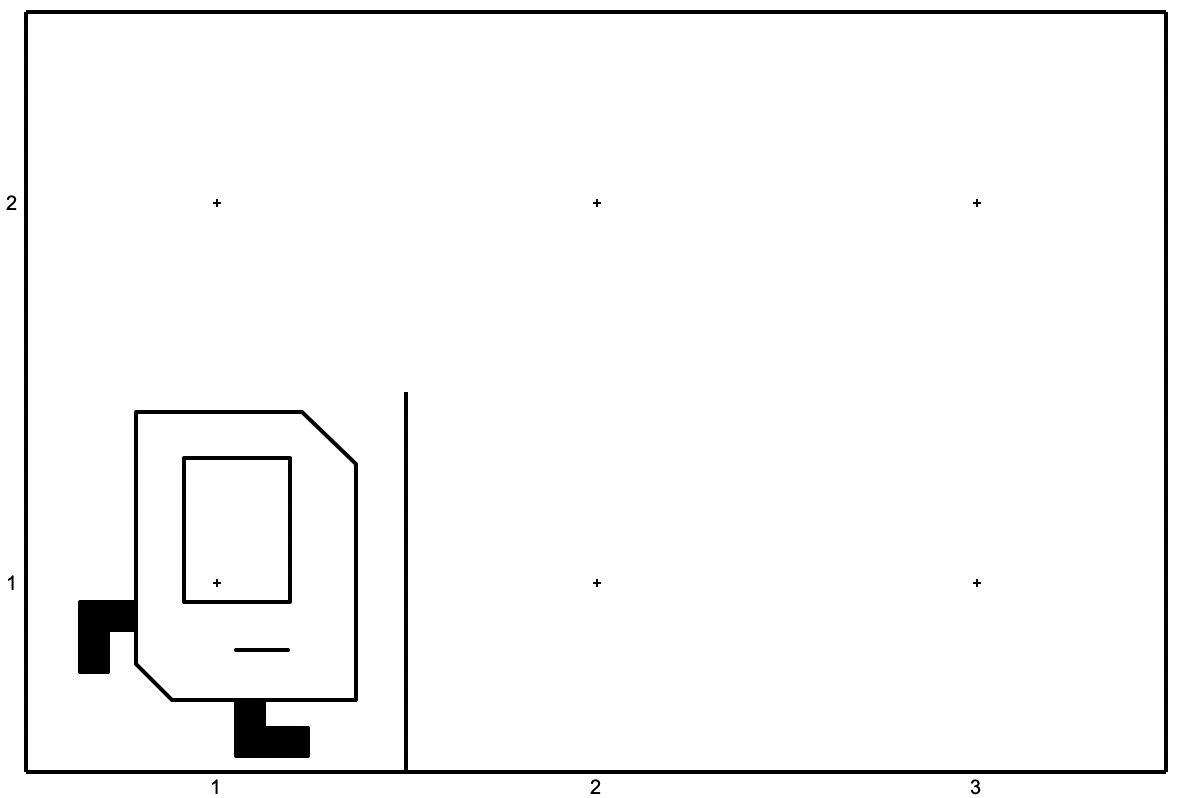
\includegraphics[width=2.5in, left]{ch02/LoopNeverEntered/init.jpg}
        \caption{}
        \label{subfig:LoopNeverEnteredA}
    \end{subfigure}
    \hspace{0.1in}
    \begin{subfigure}[t]{0.46\textwidth}
        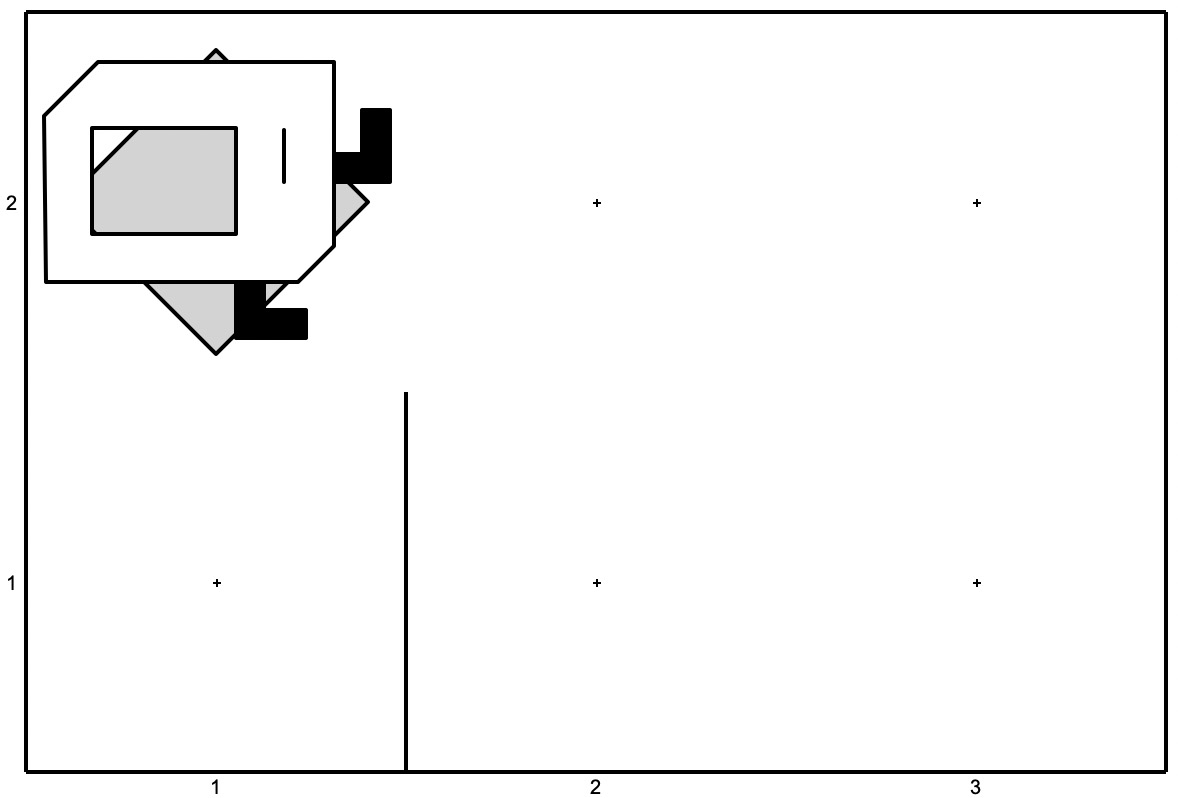
\includegraphics[width=2.5in, left]{ch02/LoopNeverEntered/final.jpg}
        \caption{}
    \end{subfigure}
    \label{fig:LoopNeverEntered}
\end{figure}

%|@{}p{4cm}@{}|@{}p{5cm}@{}|
\begin{table}
\begin{tabular}{@{}p{0.35\textwidth}@{}@{}p{0.35\textwidth}@{}}
\toprule[1.5pt]
\multicolumn{2}{c}{\mytblhdr{\myentblhdr{Karel Conditions}}}\\
\midrule
\mycode{frontIsClear()	} &	    \mycode{frontIsBlocked()   }\\
\mycode{leftIsClear()	} &		\mycode{leftIsBlocked()    }\\
\mycode{rightIsClear()	} &	    \mycode{rightIsBlocked()   }\\
\mycode{beepersPresent()} &		\mycode{noBeepersPresent() }\\
\mycode{beepersInBag()	} &	    \mycode{noBeepersInBag()   }\\
\mycode{facingNorth() 	} &	    \mycode{notFacingNorth()   }\\
\mycode{facingEast() 	} &		\mycode{notFacingEast()    }\\
\mycode{facingSouth() 	} &	    \mycode{notFacingSouth()   }\\
\mycode{facingWest() 	} &		\mycode{notFacingWest()    }\\
\bottomrule[1.5pt]
\caption{ကားရဲလ်နားလည်သော \mmCondition များ}
\label{tbl:KarelConditions}
\end{tabular}
\end{table}

\section{\mycodesecttl{if}  \myensecttl{statement}}
\enIfStatement ကို \mmcommand တွေကို အခြေအနေမှန်တော့မှ လုပ်ဆောင်စေချင်တဲ့ အခါသုံးတယ်။ \mmsyntax ကတော့ အခုလိုပုံစံ။
\begin{lstcodeminimal}
if ( (*@\myLstPlaceHolder{CONDITION}@*) ) {
        // commands to be executed if (*@\myLstPlaceHolder{CONDITION}@*) is true
}
\end{lstcodeminimal}
\noindent \myLstPlaceHolder{CONDITION} နေရာမှာ \Tbl \vref*{tbl:KarelConditions} ထဲက \mmCondition တစ်ခုကို အစားထိုးရမှာပါ။ လက်တွေ့ ဥပမာတစ်ခုကြည့်ရအောင်။ ကားရဲလ်က 

\begin{figure}[tbh!]
    \caption{\myenlstcpt{MooveMoveBeeperToOtherSide}}
    \begin{subfigure}[t]{0.46\textwidth}
        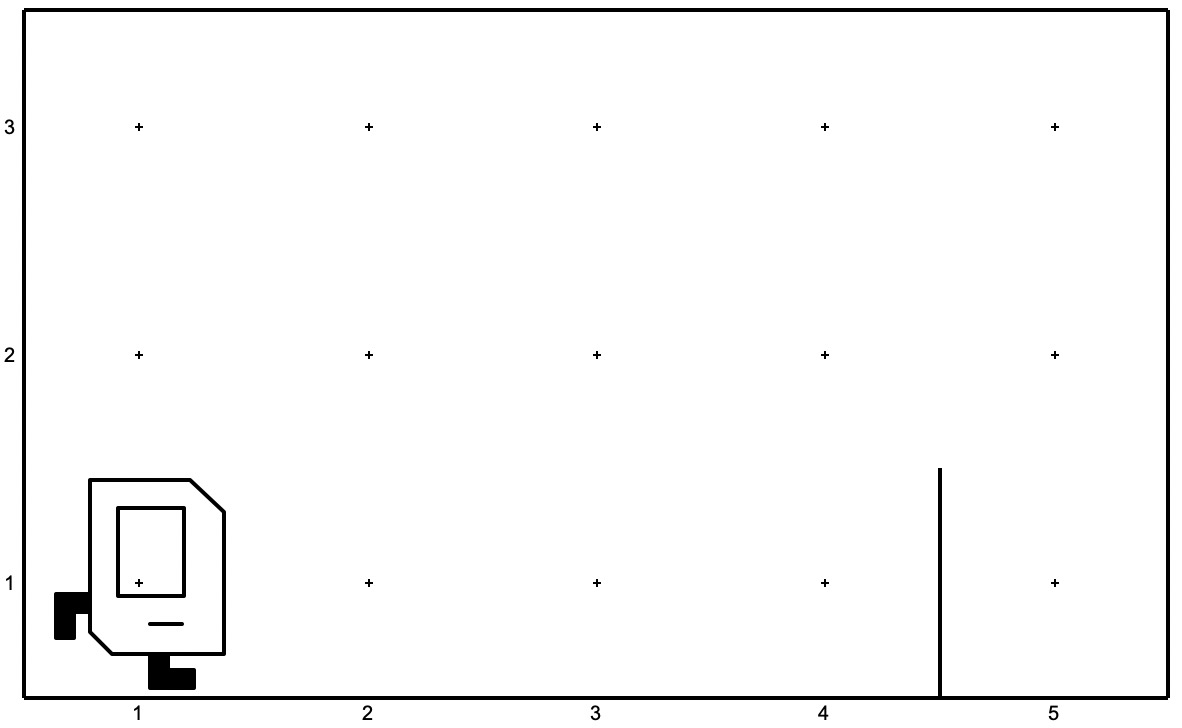
\includegraphics[width=2.5in, left]{ch02/MoveBeeperToOtherSide/init_w1.jpg}
        \caption{}
        \label{subfig:MooveMoveBeeperToOtherSideInitW1}
    \end{subfigure}
    \hspace{0.1in}
    \begin{subfigure}[t]{0.46\textwidth}
        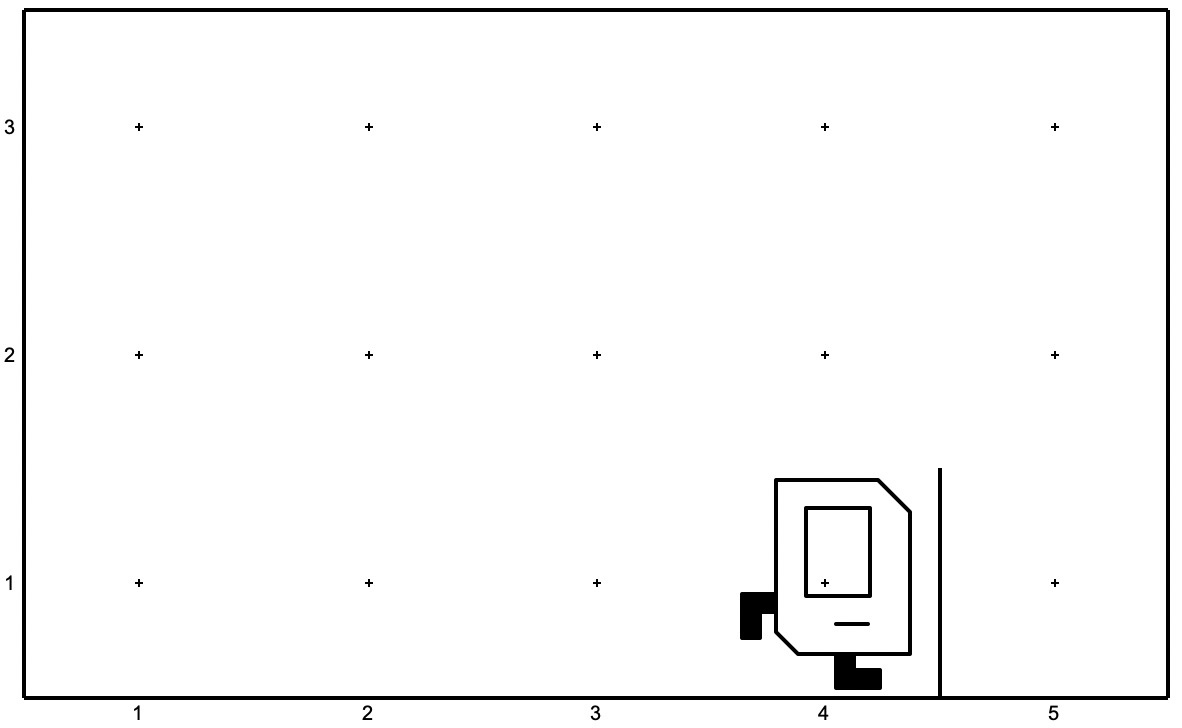
\includegraphics[width=2.5in, left]{ch02/MoveBeeperToOtherSide/final_w1.jpg}
        \caption{}
    \end{subfigure}

    \begin{subfigure}[t]{0.46\textwidth}
        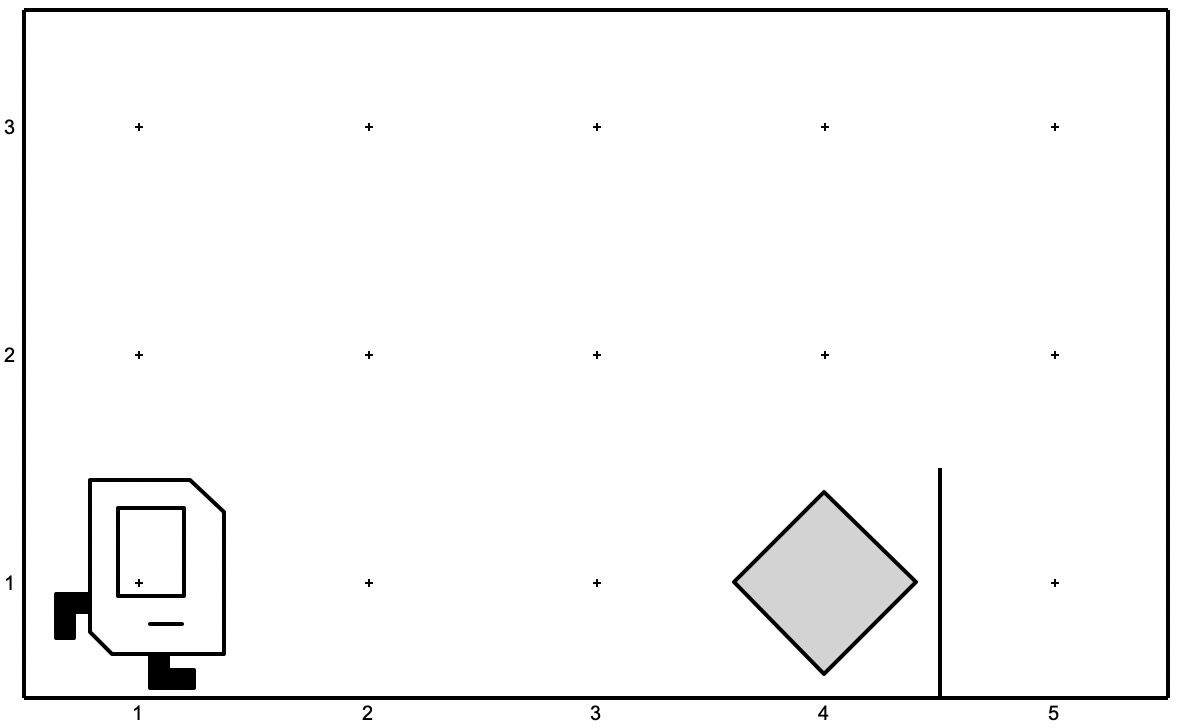
\includegraphics[width=2.5in, left]{ch02/MoveBeeperToOtherSide/init_w2.jpg}
        \caption{}
        \label{subfig:MooveMoveBeeperToOtherSideInitW2}
    \end{subfigure}
    \hspace{0.1in}
    \begin{subfigure}[t]{0.46\textwidth}
        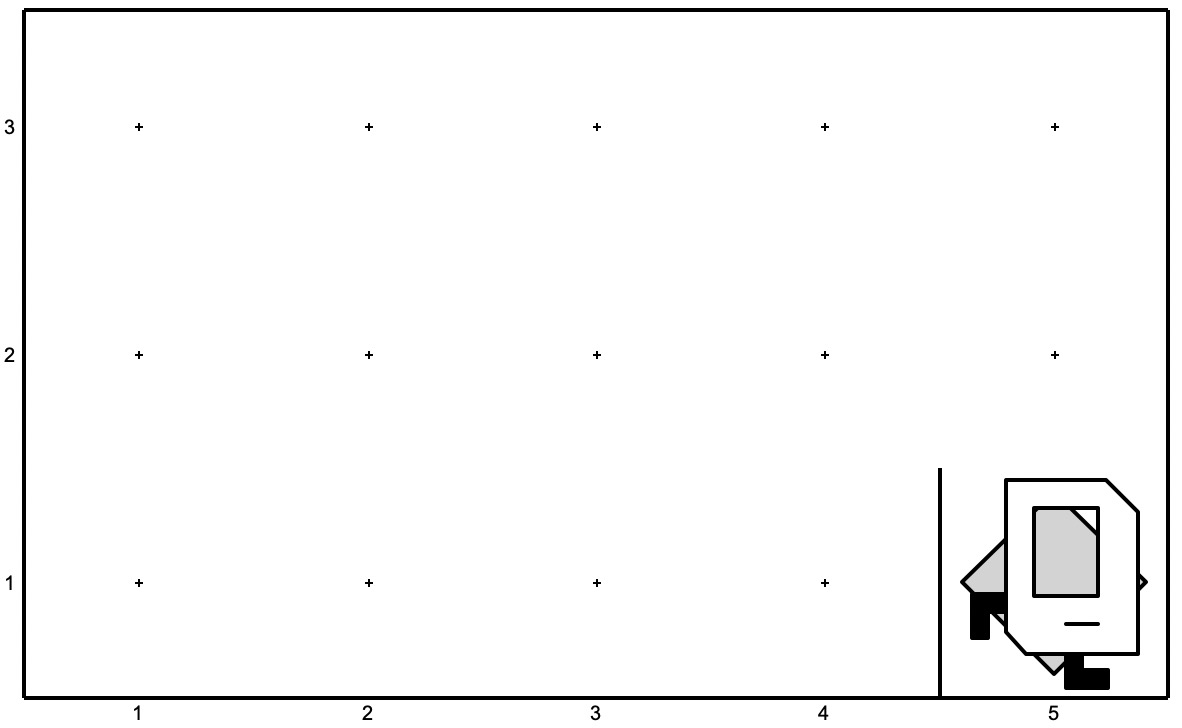
\includegraphics[width=2.5in, left]{ch02/MoveBeeperToOtherSide/final_w2.jpg}
        \caption{}
    \end{subfigure}
    \label{fig:MooveMoveBeeperToOtherSide}
\end{figure}

\begin{lstcodesimple}[float, caption={\mycodelstcpt{MoveBeeperToOtherSide.java}}, label={lst:MoveBeeperToOtherSide}]
public class MoveBeeperToOtherSide extends stanford.karel.Karel {
    public void run() {

            // Code to go pick beeper

            // Check if beeper is there and move to the other side
            if (beepersPresent()) {
                    pickBeeper();
                    turnLeft();
                    move();
                    turnRight();
                    move();
                    turnRight();
                    move();
                    putBeeper();
                    turnLeft();
            }
    }

    // turnRight method definition
}

\end{lstcodesimple}

\section{\mycodesecttl{if else}  \myensecttl{statement}}
\enIfElseStatement ကိုတော့ အခြေအနေတစ်ရပ် မှန်လျှင် လုပ်ဆောင်ချင်တာနဲ့ မှားလျှင် လုပ်ဆောင်ချင်တာ က မတူပဲကွဲပြား နေတဲ့အခါ သုံးတယ်။ \mmsyntax ကတော့ အခုလိုပုံစံ။
\begin{lstcodeminimal}
if ( (*@\myLstPlaceHolder{CONDITION}@*) ) {
        // commands to be executed if (*@\myLstPlaceHolder{CONDITION}@*) is true
} else {
        // commands to be executed if (*@\myLstPlaceHolder{CONDITION}@*) is false
}
\end{lstcodeminimal}
\noindent \myLstPlaceHolder{CONDITION} နေရာမှာ \Tbl \vref*{tbl:KarelConditions} ထဲက \mmCondition တစ်ခုကို အစားထိုးရမှာပါ။ ရှေ့မှာတွေ့ခဲ့တဲ့ ဥပမာမှာလိုပဲ \mmbeeper ရှိရင် ရွှေ့ပေးရမယ်၊ မရှိရင်တော့ စထွက်တဲ့နေရာကို ပြန်လာခိုင်းရမယ်ဆိုပါစို့။ ဒါဆိုရင် ဘိပါရှိရင် ရွှေ့ရမယ်၊ မရှိခဲ့ရင် (တနည်းအားဖြင့် beepersPresent \mmCondition ကမှားခဲ့လျှင်) ပြန်လာရမှာဖြစ်တယ်။ 

\begin{lstcodesimple}[float, caption={\mycodelstcpt{MoveBeeperToOtherSideOrComeBack.java}}, label={lst:MoveBeeperToOtherSideOrComeBack}]
public class MoveBeeperToOtherSideOrComeBack extends stanford.karel.Karel {
        public void run() {
                
                // ... 

                if (beepersPresent()) {
                        pickBeeper();
                        turnLeft();
                        move();
                        turnRight();
                        move();
                        turnRight();
                        move();
                        putBeeper();
                        turnLeft();
                } else {
                        turnLeft();
                        turnLeft();
                        move();
                        move();
                        move();
                }
        }

        // . . .turnRight method definition here
        
}
\end{lstcodesimple}

\end{sloppypar}